\section{Method}
\label{sec:method}
%\MY{We can separate things that are innovative in this section, i.e. how we ensure the patient profile quality, how we design memories and retrieve module, and how a coach/supervisor is needed to oversee the dialogue procedure. Throughout the paper, we need to say that simulating conversations between agents is difficult, and this is what differs from agent hospital paper. }

%In \system, each agent contains a chat module, a memory module, and a retrieval module. The chat module generates the response of the psychiatrist agent and patient agents based on their profile, retrieved memory, and dialogue history of the diagnosis session. The memory module of the psychiatrist agent is designed as a three-layer hierarchical memory structure to store the dialogue history, electronic medical records, summarized skills, and other information that can be leveraged in other diagnosis conversations. The supervisor plugin is designed to control the dialogue process, conclude the electronic medical records based on dialogue history and reflect the summarized skills based on the diagnosis result, aligning the psychiatrist with the real-life distribution. The retrieval module aims to retrieve the corresponding memory which can be utilized for dialogue generation and diagnosis. We will introduce the process of patients profile evaluation and the mentioned modules in detail in the following subsections.
% \MY{I've \% previous text, you can bring some back if needed.}
The complete diagnosis and reflection session can be presented in 6 stages as shown: (1) Initialize the patient agent with a profile generated through the D$^4$ dataset, and embed the ground truth diagnosis result in the patient agent. The diagnosis results of the patient agent remain unseen to the patient agent and psychiatrist agent until the predicted diagnosis result is generated. (2) The psychiatrist and the patient agent begin the conversation. (3) The supervisor plugin updates the diagnosis tracking list, provides next-turn instruction based on the dialogue history and diagnosis tracking list, and stimulates conversation of the next round. The step (2) and (3) repeat until the conversation finish. (4) After the conversation, the psychiatrist agent generates the electronic medical records and the diagnosis result. The supervisor plugin compares the ground truth diagnosis result and the diagnosis result generated by the psychiatrist agent, and reflects the skills if the generated results are not correct. (5) The supervisor plugin updates the summarized skills in the memory module of the psychiatrist agent, and (6) The psychiatrist agent calls the next patient and repeats the whole procedure.
To improve dialogue quality and diagnosis accuracy, each agent contains a chat module, a memory module, and a retrieval module. Psychiatrist's memory is a newly proposed tertiary memory framework. Each module will be introduced in detail.

\subsection{Chat Module}
The chat module takes the profile of the agent, relevant memory retrieved, and dialogue history as input, and generates the utterance that the agent going to say. Since the psychiatrist always plays a proactive role during the diagnosis conversation, we take advantage of the supervisor plugin 
%\KZ{Instead of ``coach plugin'', maybe call it ``dialogue control unit''.}
of the psychiatrist agent to control the dialogue process. The dialogue generation function used in step (2) of Figure~\ref{fig:overview} can be presented in Equation~\ref{eq:dialogue generation}. The $\mathrm{PPT}_d$, $\mathrm{PRF}$ indicates the constant prompt and personal profile utilized for dialogue generation, respectively, the $\mathrm{mem}$ suggests the retrieved memory, $\mathrm{ins}$ means the instruction generated by supervisor plugin, only provided if the profile is the psychiatrist agent, and the $\mathrm{utt}_{:i-1}$ is the dialogue history until now. 

\begin{equation}
    \mathrm{utt}_{i} = \mathrm{LLM}(\mathrm{PPT}_d, \mathrm{PRF}, \mathrm{mem}, [\mathrm{ins}],\mathrm{utt}_{:i-1})
    \label{eq:dialogue generation}
\end{equation}

The diagnosis function is attached in the chat module. The diagnosis function takes the whole dialogue history and relevant memory retrieved as input, and generates the detailed diagnosed symptoms and the predicted depression risk and suicide risk. The diagnosis function can be presented in Equation~\ref{eq:diagnosis}. The $\mathrm{PPT}_{diag}$ indicates the constant prompt utilized for diagnosis result generation. Since the response from LLM is always unstable, it results in bias during the experiments. Therefore, we apply a voting diagnosis method. To be specific, we let the LLM generate $k$ samples of diagnosis response ($k=5$ in our experiments). After that, we map the depression risk and suicide risk to integer: control(0), mild(1), moderate(2), and severe(3) as shown in Equation~\ref{eq:vote}. We get the most voted risk level in most cases. If tie, we choose the rounded average of all votes as the final decision. 

\begin{equation}
    \mathrm{diag}_i = \mathrm{LLM}(\mathrm{PPT}_{diag}, \mathrm{PRF}, \mathrm{mem}, \mathrm{utt}_{:})
    \label{eq:diagnosis}
\end{equation}
\begin{equation}
\mathrm{diag}=\begin{cases}
      \mathrm{mode}(\{\mathrm{diag}_i\}_k), & \text{if only one mode exists} \\ 
      \mathrm{average}(\{\mathrm{diag}_i\}_k), & \text{otherwise}
    \end{cases}
\label{eq:vote}
\end{equation}

After the conversation, the chat module summarizes the dialogue history as EMR, including all the symptoms and their severity mentioned in the dialogue. The function is presented in Equation~\ref{eq:EMR generation}, the $\mathrm{PPT}_{emr}$ represents the constant prompt utilized for concluding EMR.

\begin{equation}
    \mathrm{EMR} = \mathrm{LLM}(\mathrm{PPT}_{emr}, \mathrm{utt}_{:})
    \label{eq:EMR generation}
\end{equation}

\subsection{Tertiary Memory Mechanism}

Memory module is provided as an external storage space to overcome the limitation of input length of LLMs~\cite{zhang2024surveymemorymechanismlarge}. The previous memory structure~\cite{Park2023GenerativeAgents} regards memory nodes as equal nodes, which is not appropriate in more complex scenarios. Although some works have proposed multi-layer memory structures~\cite{qian2024chatdevcommunicativeagentssoftware,li2023tradinggptmultiagentlayeredmemory,sumers2023cognitive, maharana2024evaluatinglongtermconversationalmemory}, they are still underexplored, as they are based merely on the long-short memory concept without a specific division of roles across different memory layers. To fully simulate the process of psychiatrist training in a real-life scenario, we design a three-level hierarchical memory structure consisting of \textit{Conversation Records, Electronic Medical Records, and Diagnostic Skills}, 
which mimics the exact training process of a psychiatrist, where useful information is extracted into EMR during a patient counseling session, and as their experiences with more patients accumulate, their clinical and diagnostic skills are elevated.  %We will describe the memory layers in detail.

\begin{itemize}
    \item \textbf{Conversation Records} represent the pure transcripts of the diagnosis conversation between patient agents and psychiatrist agents. It helps the psychiatrist agent to conclude the electronic medical records of the patient agents. 
    \item \textbf{Electronic Medical Records (EMR)} indicate the summary of the patients' portrait, chief complaint, and symptom list. EMR can be leveraged as a summary of specific diagnosis sessions, which can be utilized by psychiatrists to search for similar cases and summarized skills.
    \item\textbf{Diagnostic Skills} play as the optimizer in training psychiatrist agents. Summarized Skills take the dialogue history, diagnosis result generated by the psychiatrist agent, and the ground truth diagnosis result given by a professional psychiatrist in real life in D$^4$ as input, while output summarized skills mainly focus on what kind of symptoms are overestimated or underestimated during diagnosis procedure, guide the LLM-powered psychiatrist agent towards professional psychiatrists. Summarized skills help the psychiatrist agent to imitate the real-world distribution.
\end{itemize}

\begin{figure}[!t]
    \centering
    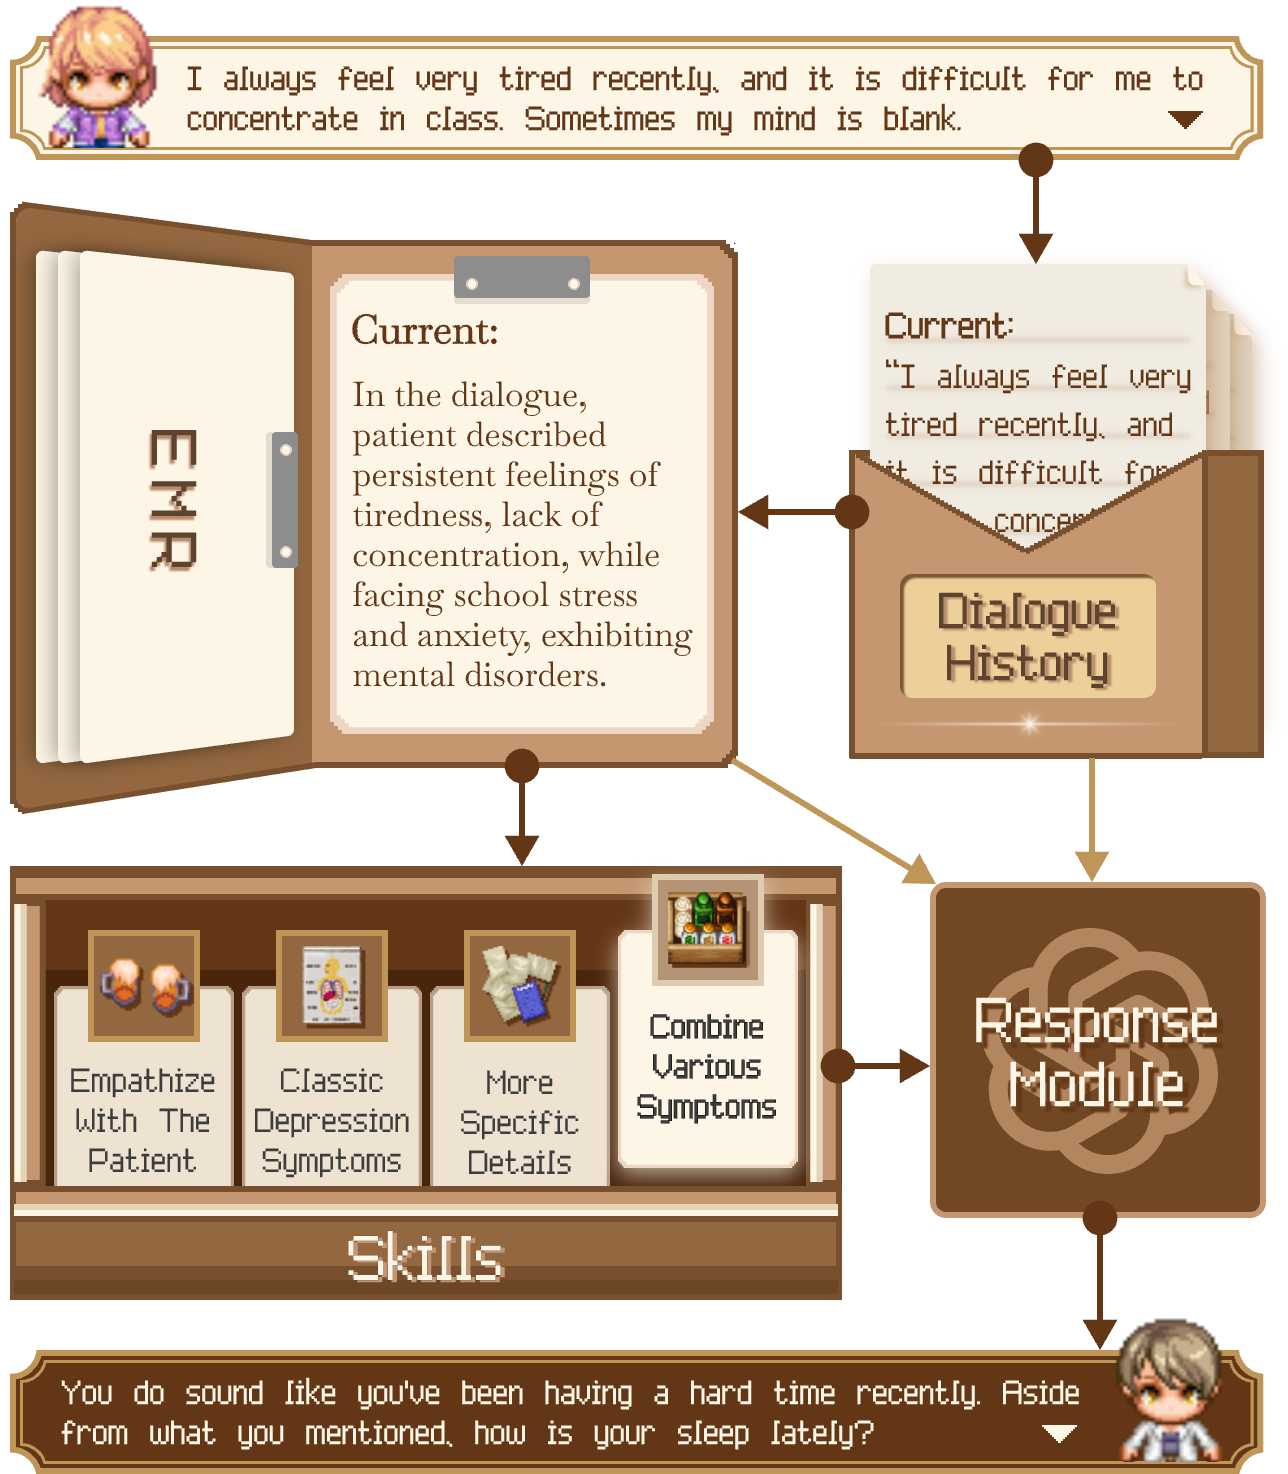
\includegraphics[width=1\linewidth]{fig/memory.png}
    \caption{\textbf{The Tertiary Memory Structure of \system.} The utterance of the diagnosis conversation will be stored in \textbf{Dialogue History}. The whole dialogue history in the session will be summarized into electronic medical records (\textbf{EMR}). \textbf{Skills} are generated by the supervisor plugin. All the memory will contribute to the dialogue generation.}
    \label{fig:memory structure}
\end{figure}

As illustrated in Figure~\ref{fig:memory structure}, these three tiers of memory mechanisms constitute a progression from the most fundamental and granular level, through abstraction, to the most condensed, compressed, and consequently, more enduring form. Each subsequent layer represents a refinement process where information is distilled from its original detailed state into a more concise and long-lasting representation. This hierarchical organization enables the psychiatrist system to not only store vast amounts of data efficiently but also retrieve it effectively over time, as the most essential elements are preserved in the most refined and enduring form.
%\MY{can you put these text into a figure, just using 3 text blocks with arrows in between, then you can save space here, i'll send you a scratch. also maybe just clinical skills, or diagnosis skills, not summarized skills}

\subsection{Supervisor Plugin of the Psychiatrist Agent}
%\MY{or maybe a supervisor shadow?}
The supervisor plugin tracks the symptoms mentioned by the patient agent and maintains a detailed symptom list, where each symptom is assigned one of three statuses: unknown, true, or false. Meanwhile, the supervisor plugin updates the list based on the dialogue history, and also provides the question list psychiatrist agents need to ask in the next round, avoiding repeatedly asking similar questions but focusing on those unknown symptoms, which enhances the effectiveness of the diagnosis conversation. The supervisor plugin also controls the dialogue stage change as we define three stages of the diagnosis dialogue:
\begin{itemize}
    \item \textbf{Start Stage}: The start stage aims to start the diagnosis conversation session, mainly focusing on asking the chief complaints of the patient agents and building a healthy therapeutic alliance~\cite{Horvath2011AllianceII} with them. 
    \item \textbf{Exploring Stage}: The exploring stage aims to collect detailed information of the patient agents, and tries to find out the most effective way to complete the diagnosis session.
    \item \textbf{End Stage}: The end stage aims to finish the dialogue, summarizes the information collected, and gives some advice to the patient agents based on the dialogue history. 
\end{itemize}

The instruction generation function of the supervisor plugin can be presented in Equation~\ref{eq:instruction generation}. The $\mathrm{PPT}_ins$ implies the constant prompt utilized in the instruction generation.

\begin{equation}
    \mathrm{ins}_{i}, \mathrm{stat}_i = \mathrm{LLM}(\mathrm{PPT}_c, \mathrm{PRF}, \mathrm{stat}_{i-1}, \mathrm{utt}_{:i-1})
    \label{eq:instruction generation}
\end{equation}

The supervisor plugin also acts as a teacher to generate skills based on the ground truth diagnosis result and the generated diagnosis result based on the dialogue history. The skill generation function is represented in Equation \ref{eq:skill generation}. $\mathrm{PPT}_s$ implies the constant prompt utilized for reflecting skills, $\hat{\mathrm{diag}}$ means the ground truth diagnosis result provided by the supervisor, based on annotation on D$^4$ dataset.

\begin{equation}
    \mathrm{Skills} = \mathrm{LLM}(\mathrm{PPT}_s, \mathrm{PRF}, \mathrm{utt}_{:}, \hat{\mathrm{diag}}, \mathrm{diag})
    \label{eq:skill generation}
\end{equation}
% \begin{table*}[h!]
%     \centering
%     \setlength{\tabcolsep}{3pt}
%     \begin{tabular}{cccccccccc}
%         \toprule
%         \multirow{2.5}{*}{\textbf{Setting}} & \multirow{2.5}{*}{\textbf{Memory}} & \multicolumn{4}{c}{\textbf{Original Dialogues}} & \multicolumn{4}{c}{\textbf{Simulated Dialogues}} \\
%         \cmidrule(rl){3-6}\cmidrule(rl){7-10}
%         &            & Dep. & Su. & Sym. & \textbf{Overall} & Dep. & Su. & Sym. & \textbf{Overall} \\
%         \midrule
%         \multirow{2}{*}{\makecell[c]{\textbf{Quiz}\\(Train)}}  & w/o &  41.0    &   49.8  &  40.2    &    \cellcolor{gray!30}43.7     & 21.8  &    23.4  &   35.2  &   \cellcolor{gray!30}26.8     \\
%                                         & w/ & 48.2(+7.2)  & 51.4(+1.6)  & 40.8(+0.6)  & \cellcolor{gray!30}46.8(+3.1)     & 27.6(+5.8)  & 26.4(+3.0)  & 37.2(+1.6)  & \cellcolor{gray!30}30.4(+3.6)     \\
%         \midrule
%         \multirow{2}{*}{\makecell[c]{\textbf{Exam}\\(Test)}}   & w/o  &  28.0    &   26.0   &  36.2    &  \cellcolor{gray!30}30.1       &  16.4    &    12.0  &  34.2    &  \cellcolor{gray!30}20.9       \\
%                                         & w/ & 32.4 (+4.4)  & 27.0 (+1.0)  & 35.0 (-1.2)  & \cellcolor{gray!30} 31.5(+1.4)     & 23.2(+6.8)  & 13.6(+1.6)  & 34.2(-)  & \cellcolor{gray!30}23.7(+2.8)     \\
%         \bottomrule
%     \end{tabular}
%     \caption{\textbf{The main experiment results on depression diagnosis.} Dep. : the accuracy of depression risk classification. Su. : the accuracy of suicide risk classification. Sym. : the average accuracy of symptom prediction.}
    %\MY{I still think we should change them as seen, unseen cases. For both settings, they are trained on the same training set, but evaluating on seen and unseen cases right}}
    % (Ref): enable reflection if the prediction of the first attempt is incorrect, this is not adopted in the test set.
%     \label{tab:main}
% \end{table*}

\begin{table*}[h!]
    \centering
    % \setlength{\tabcolsep}{4pt}
    \begin{tabular}{cccccccc}
        \toprule
        \multirow{2.5}{*}{\textbf{Setting}} & \multirow{2.5}{*}{\textbf{Memory}} & \multicolumn{3}{c}{\textbf{Original Dialogues}} & \multicolumn{3}{c}{\textbf{Simulated Dialogues}} \\
        \cmidrule(rl){3-5}\cmidrule(rl){6-8}
        &            & Dep. & Su. & \textbf{Overall} & Dep. & Su. & \textbf{Overall} \\
        \midrule
        \multirow{2}{*}{\makecell[c]{\textbf{Quiz}\\(Train)}}  & w/o &  41.0    &   49.8  & \cellcolor{gray!30}45.4     & 21.8  &    23.4  & \cellcolor{gray!30}22.6     \\
                                        & w/ & 48.2(+7.2)  & 51.4(+1.6)  & \cellcolor{gray!30}49.8(+4.4)     & 27.6(+5.8)  & 26.4(+3.0)  & \cellcolor{gray!30}27.0(+4.4)     \\
        \midrule
        \multirow{2}{*}{\makecell[c]{\textbf{Exam}\\(Test)}}   & w/o  &  28.0    &   26.0   & \cellcolor{gray!30}27.0       &  16.4    &    12.0  & \cellcolor{gray!30}14.2       \\
                                        & w/ & 32.4 (+4.4)  & 27.0 (+1.0)  & \cellcolor{gray!30}29.7(+2.7)     & 23.2(+6.8)  & 13.6(+1.6)  & \cellcolor{gray!30}18.4(+4.2)     \\
        \bottomrule
    \end{tabular}
    \caption{\textbf{The main experiment results on depression diagnosis.} Dep. : the accuracy of depression risk classification. Su. : the accuracy of suicide risk classification.}
    \label{tab:main}
\end{table*}




\subsection{Retrieval Module}
The retrieval module aims to search for helpful electronic medical records and summarized skills, to better generate responses and diagnosis results. The retrieval module is also responsible for the reassignment of the memory nodes, based on the diagnosis result. We modify the classical retrieve score calculation function~\cite{Park2023GenerativeAgents}. However, since our system does not simulate the time step of the diagnosis, we do not apply the calculation of recency in our experiment. Therefore, we mainly calculate relevance score and importance score. The relevance score is calculated as $\mathrm{rel} = \mathrm{NORM}(\mathrm{E}(\mathrm{mem})\cdot \mathrm{E}(\mathrm{query}))$. $\mathrm{NORM}$ indicates min-max scaling method for normalization. $\mathrm{E}$ represents the embedding model, and $\mathrm{query}$ suggests the last utterance during the diagnosis conversation, and the concluded EMR of the dialogue during the diagnosis. The importance score $\mathrm{imp}$ is set to 5 when the memory node is generated, and updates based on the diagnosis results, which suggests the effectiveness of the according memory. The importance score also applies min-max scaling normalization during calculation. Specifically, if the diagnosis result matches the ground truth, the importance score will be increased by one; if it does not, the score will be decreased by one. The final score is calculated as the weighted sum of relevance score $\mathrm{score} = \alpha_1 \mathrm{rel} + \alpha_2 \mathrm{imp}$, while $\alpha_s$ are set to 1 in our experiments. Meanwhile, our observations during the experiments indicate that if we utilize the mere top-$k$ retrieve method as prior work~\cite{Park2023GenerativeAgents} utilized, the memory node retrieved does not vary much with the experiment going, since the top-$k$ memory nodes are fixed. Therefore, we apply a sampling memory retrieval method in the retrieval module. To be specific, we normalize the retrieval score into a probability distribution, which can be seen in Equation~\ref{eq:probability}. After normalizing the score, the retrieval module selects $k$ memory nodes based on the probability distribution. $k$ is set to 10 in our experiment setting. 

\begin{equation}
    p_i = \frac{\mathrm{socre}_i}{\sum_j \mathrm{score}_j}
    \label{eq:probability}
\end{equation}